\section*{Problema 1}
Dada la ecuación diferencial
\begin{equation}
	y^{\prime} (x) = y^2 + 1, \label{dif1}
\end{equation}
en la región $0 < x < 1$ con condiciones iniciales $y(0) = 0$. Utilizando el método de Euler, se encuentra la solución a \eqref{dif1} con diferentes tamaños de paso, con los que se encuentran el número de iteraciones\footnote{Dado un tamaño de paso y un intervalo se encuentra el número de iteraciones con la fórmula $n = (b - a)/h$.}. 

Utilizando los resultados y la solución real de la ecuación diferencial se obtiene la figura \ref{ej1}.
\begin{figure}[H]
	\centering
	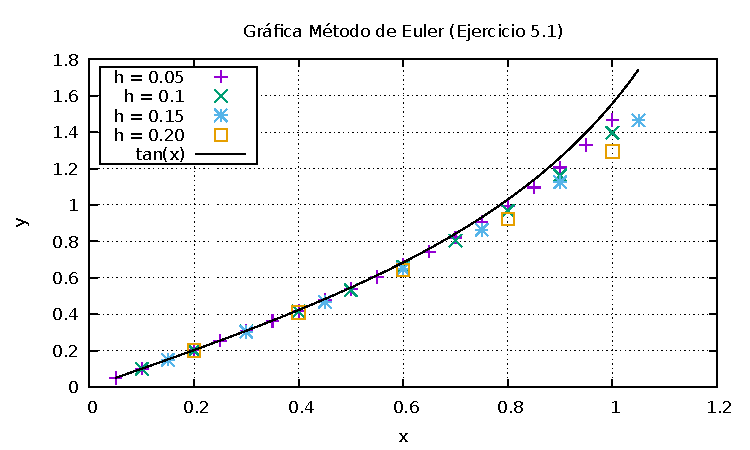
\includegraphics[scale=1]{../img/ej5-1.pdf}
	\caption{Gráfica para diferentes tamaños de paso.}
	\label{ej1}
\end{figure}

El código creado para la solución es:
\begin{lstlisting}
// Librerias
#include <iostream>
#include <fstream>

using namespace std;

double euler(double y, double x, double h);
double derivada(double y, double x);


int main(){
  const double y0 = 0.0;
  const double x0 = 0.0;
  const double h [4] = {0.05,0.10,0.15,0.20};
  const int N [4] = {20,10,7,5};
  ofstream salida_uno, salida_dos, salida_tres, salida_cuatro;


  double y = y0;
  double x = x0;
  double y_new = 0.0;

  // METODO DE EULER Y GENERACION DE ARCHIVOS
  salida_uno.open("h1.dat", ios::out);
  for(int i = 0; i <= N[0] - 1; i++){
    y_new = euler(y, x, h[0]);

    y = y_new;
    x = x + h[0];

    salida_uno << x << "\t" << y << endl;
  } // END FOR
  salida_uno.close();


  y = y0;
  x = x0;
  y_new = 0.0;
  salida_dos.open("h2.dat", ios::out);
  for(int i = 0; i <= N[1] - 1; i++){
    y_new = euler(y, x, h[1]);

    y = y_new;
    x = x + h[1];

    salida_dos << x << "\t" << y << endl;
  } // END FOR
  salida_dos.close();


  y = y0;
  x = x0;
  y_new = 0.0;
  salida_tres.open("h3.dat", ios::out);
  for(int i = 0; i <= N[2] - 1; i++){
    y_new = euler(y, x, h[2]);

    y = y_new;
    x = x + h[2];

    salida_tres << x << "\t" << y << endl;
  } // END FOR
  salida_tres.close();


  y = y0;
  x = x0;
  y_new = 0.0;
  salida_cuatro.open("h4.dat", ios::out);
  for(int i = 0; i <= N[3] - 1; i++){
    y_new = euler(y, x, h[3]);

    y = y_new;
    x = x + h[3];

    salida_cuatro << x << "\t" << y << endl;
  } // END FOR
  salida_cuatro.close();

  return 0;
} // END MAIN


double euler(double y, double x, double h){
  return y + h*derivada(y,x);
} // END EULER


double derivada(double y, double x){
  return y*y + 1;
} // END DERIVADA
\end{lstlisting}

\section*{Problema 2}
Para la misma ecuación diferencial \eqref{dif1}, se compararon los resultados entre el Método de Euler, el Método de Euler Modificado y el Método de Euler Mejorado. Esto, únicamente, con $h = 0.1$ como tamaño de paso. Entonces, la solución encontrada para cada uno de los métodos se muestra en la figura \ref{ej2}.

\begin{figure}[H]
	\centering
	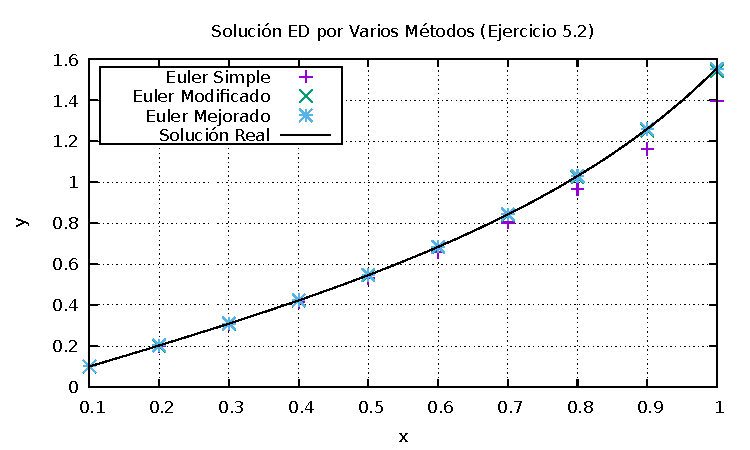
\includegraphics[scale=1]{../img/ej5-2.pdf}
	\caption{Gráfica de los distintos métodos de Euler para la ecuación \eqref{dif1}.}
	\label{ej2}
\end{figure}


El código creado para la solución es:
\begin{lstlisting}
// Librerias
#include <iostream>
#include <fstream>

using namespace std;


double euler(double y, double x, double h);
double euler_modificado(double y, double x, double h);
double euler_mejorado(double y, double x, double h);
double derivada(double y, double x);


int main(){
  const double y0 = 0.0;
  const double x0 = 0.0;
  const double h = 0.10;
  const int N = 10;
  ofstream salida_simple, salida_mejorado, salida_modificado;

  double y = y0;
  double x = x0;
  double y_new = 0.0;


  salida_simple.open("simple.dat", ios::out);
  for (int i = 0; i <= N - 1; i++){
    y_new = euler(y, x, h);

    y = y_new;
    x = x + h;

    salida_simple << x << "\t" << y << endl;
  } // END FOR
  salida_simple.close();


  y = y0;
  x = x0;
  y_new = 0;
  salida_modificado.open("modificado.dat", ios::out);
  for (int i = 0; i <= N - 1; i++){
    y_new = euler_modificado(y, x, h);

    y = y_new;
    x = x + h;

    salida_modificado << x << "\t" << y << endl;
  } // END FOR
  salida_modificado.close();


  y = y0;
  x = x0;
  y_new = 0;
  salida_mejorado.open("mejorado.dat", ios::out);
  for (int i = 0; i <= N - 1; i++){
    y_new = euler_mejorado(y, x, h);

    y = y_new;
    x = x + h;

    salida_mejorado << x << "\t" << y << endl;
  } // END FOR
  salida_mejorado.close();

  return 0;
} // END MAIN

double euler(double y, double x, double h){
  return y + h*derivada(y,x);
} // END EULER

double euler_modificado(double y, double x, double h){
  double x_mid = x + 0.5*h;
  double y_mid = y + 0.5*h*derivada(y, x);
  return y + h*derivada(y_mid, x_mid);
} // END EULER_MODIFICADO

double euler_mejorado(double y, double x, double h){
  double y_tilde = y + h*derivada(y, x);
  double y_imas1 = y + 0.5*h*( derivada(y, x) + derivada(y_tilde, x + h) );
  return y_imas1;
} // END EULER_MEJORADO


double derivada(double y, double x){
  return y*y + 1;
} // END DERIVADA

\end{lstlisting}



\section*{Problema 3}








%%%%%%%